% This file was created by tikzplotlib v0.9.8.
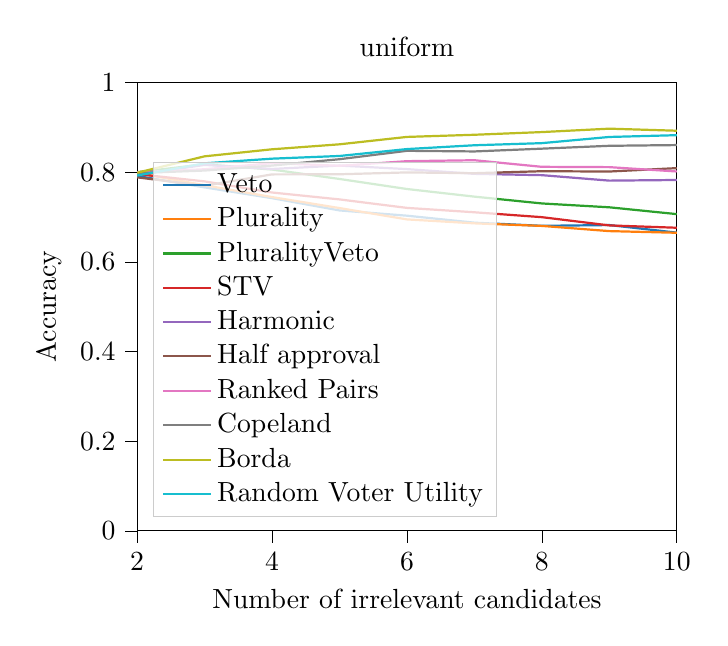
\begin{tikzpicture}

\definecolor{color0}{rgb}{0.12156862745098,0.466666666666667,0.705882352941177}
\definecolor{color1}{rgb}{1,0.498039215686275,0.0549019607843137}
\definecolor{color2}{rgb}{0.172549019607843,0.627450980392157,0.172549019607843}
\definecolor{color3}{rgb}{0.83921568627451,0.152941176470588,0.156862745098039}
\definecolor{color4}{rgb}{0.580392156862745,0.403921568627451,0.741176470588235}
\definecolor{color5}{rgb}{0.549019607843137,0.337254901960784,0.294117647058824}
\definecolor{color6}{rgb}{0.890196078431372,0.466666666666667,0.76078431372549}
\definecolor{color7}{rgb}{0.737254901960784,0.741176470588235,0.133333333333333}
\definecolor{color8}{rgb}{0.0901960784313725,0.745098039215686,0.811764705882353}

\begin{axis}[
legend cell align={left},
legend style={
  fill opacity=0.8,
  draw opacity=1,
  text opacity=1,
  at={(0.03,0.03)},
  anchor=south west,
  draw=white!80!black
},
tick align=outside,
tick pos=left,
title={uniform},
x grid style={white!69.0196078431373!black},
xlabel={Number of irrelevant candidates},
xmin=2, xmax=10,
xtick style={color=black},
y grid style={white!69.0196078431373!black},
ylabel={Accuracy},
ymin=0, ymax=1,
ytick style={color=black}
]
\addplot [thick, color0]
table {%
2 0.7916
3 0.766
4 0.742
5 0.7146
6 0.7029
7 0.6873
8 0.6803
9 0.682
10 0.6651
};
\addlegendentry{Veto}
\addplot [thick, color1]
table {%
2 0.7981
3 0.7709
4 0.7444
5 0.7199
6 0.6946
7 0.6858
8 0.6801
9 0.6685
10 0.6648
};
\addlegendentry{Plurality}
\addplot [thick, color2]
table {%
2 0.7999
3 0.8175
4 0.8058
5 0.7848
6 0.7624
7 0.7454
8 0.7302
9 0.7216
10 0.7064
};
\addlegendentry{PluralityVeto}
\addplot [thick, color3]
table {%
2 0.7956
3 0.7794
4 0.7546
5 0.7392
6 0.7203
7 0.7105
8 0.6996
9 0.6812
10 0.676
};
\addlegendentry{STV}
\addplot [thick, color4]
table {%
2 0.794
3 0.8162
4 0.8071
5 0.8147
6 0.8068
7 0.7962
8 0.7933
9 0.7811
10 0.7825
};
\addlegendentry{Harmonic}
\addplot [thick, color5]
table {%
2 0.7884
3 0.7697
4 0.795
5 0.7953
6 0.7994
7 0.7977
8 0.8021
9 0.8014
10 0.809
};
\addlegendentry{Half approval}
\addplot [thick, color6]
table {%
2 0.7998
3 0.8065
4 0.8201
5 0.8142
6 0.8245
7 0.8266
8 0.8119
9 0.8112
10 0.8015
};
\addlegendentry{Ranked Pairs}
\addplot [thick, white!49.8039215686275!black]
table {%
2 0.7979
3 0.8036
4 0.8147
5 0.8289
6 0.8476
7 0.8462
8 0.8524
9 0.8588
10 0.8604
};
\addlegendentry{Copeland}
\addplot [thick, color7]
table {%
2 0.7987
3 0.8353
4 0.851
5 0.8621
6 0.8786
7 0.8834
8 0.8894
9 0.897
10 0.8924
};
\addlegendentry{Borda}
\addplot [thick, color8]
table {%
2 0.7925
3 0.8197
4 0.8301
5 0.8361
6 0.8515
7 0.86
8 0.8647
9 0.8785
10 0.8825
};
\addlegendentry{Random Voter Utility}
\end{axis}

\end{tikzpicture}
